\chapter{System Implementation} \label{chap:sysImplementation}
%\version{v1.10.2015}

\section{System Architecture}
Pet Diet and Health care planner consists of android application and as well as web application. The android application will generate the pet diet plan, pet diseases details, diet notification alarm and doctor appointment. Pet diet plans are saved into the cloud base database and that are retrieve on the basis of pet age, specie and kind of breed. Diseases details will be shown on the basis of pet specie.\par Notification alarm will be generated on the proper timings within a day. Email will send on time when the user click on the appointment button in android application. The web application will display the hospital information like hospital services and doctors.

\section{Tools and Technology Used}
\begin{enumerate}
\item \textbf{Microsoft office}\\Microsoft office is used for project documentation and presentation. Microsoft Visio is useful for designing flow charts, activity and system diagrams.
\item \textbf{Adobe Photoshop for designing}\\Adobe photo shop is very helpful for designing the mobile application layouts, compressing the images size and increasing the resolution.
\item \textbf{Canva online designing tool}\\Canva is the online tool for graphics. The tool has been used for shades and image transparency.
\end{enumerate}


\subsection{Developers Tools}
\begin{enumerate}
\item \textbf{Android studio 3.0.1}\\
Currently the most stable version of android studio is android studio 3.0.1. Provide many facilities like latest use of libraries and API’s.
\item \textbf{Firebase  database}\\
Firebase is GOOGLE supported Cloud base platform. It is highly flexible and responsive. Providing user authentication, storage and hosting etc.
\item \textbf{Sublime Text3}\\
Sublime Text3 tool is used in developing web pages.
\end{enumerate}
\subsection{Languages Used}
\begin{enumerate}
\item \textbf{html, css, bootstrap }
      Web application is developed under html, css, and bootstrap and java script.
\item \textbf{Java}
      Android mobile application support java.
\item \textbf{Xml}
     Android studio support XML for designing application layouts or mockups.
\item \textbf{html, css, bootstrap }
      Web application is developed under html, css, and bootstrap and java script.
\item \textbf{Java}
      Android mobile application support java.
\item \textbf{Xml}
     Android studio support XML for designing application layouts or mockups.
\end{enumerate}

\section{Processing Logic}
Firstly user will login into the android app then user can view the main home activity. User can input the information related to pet specie, breed and age and then view the detail which is generated by the firebase database. User can generate the food timing notification alarm to feed his/her pet on time. Appointment can be taken through android and as well as through the website user.
\begin{figure}[H]
\centering
  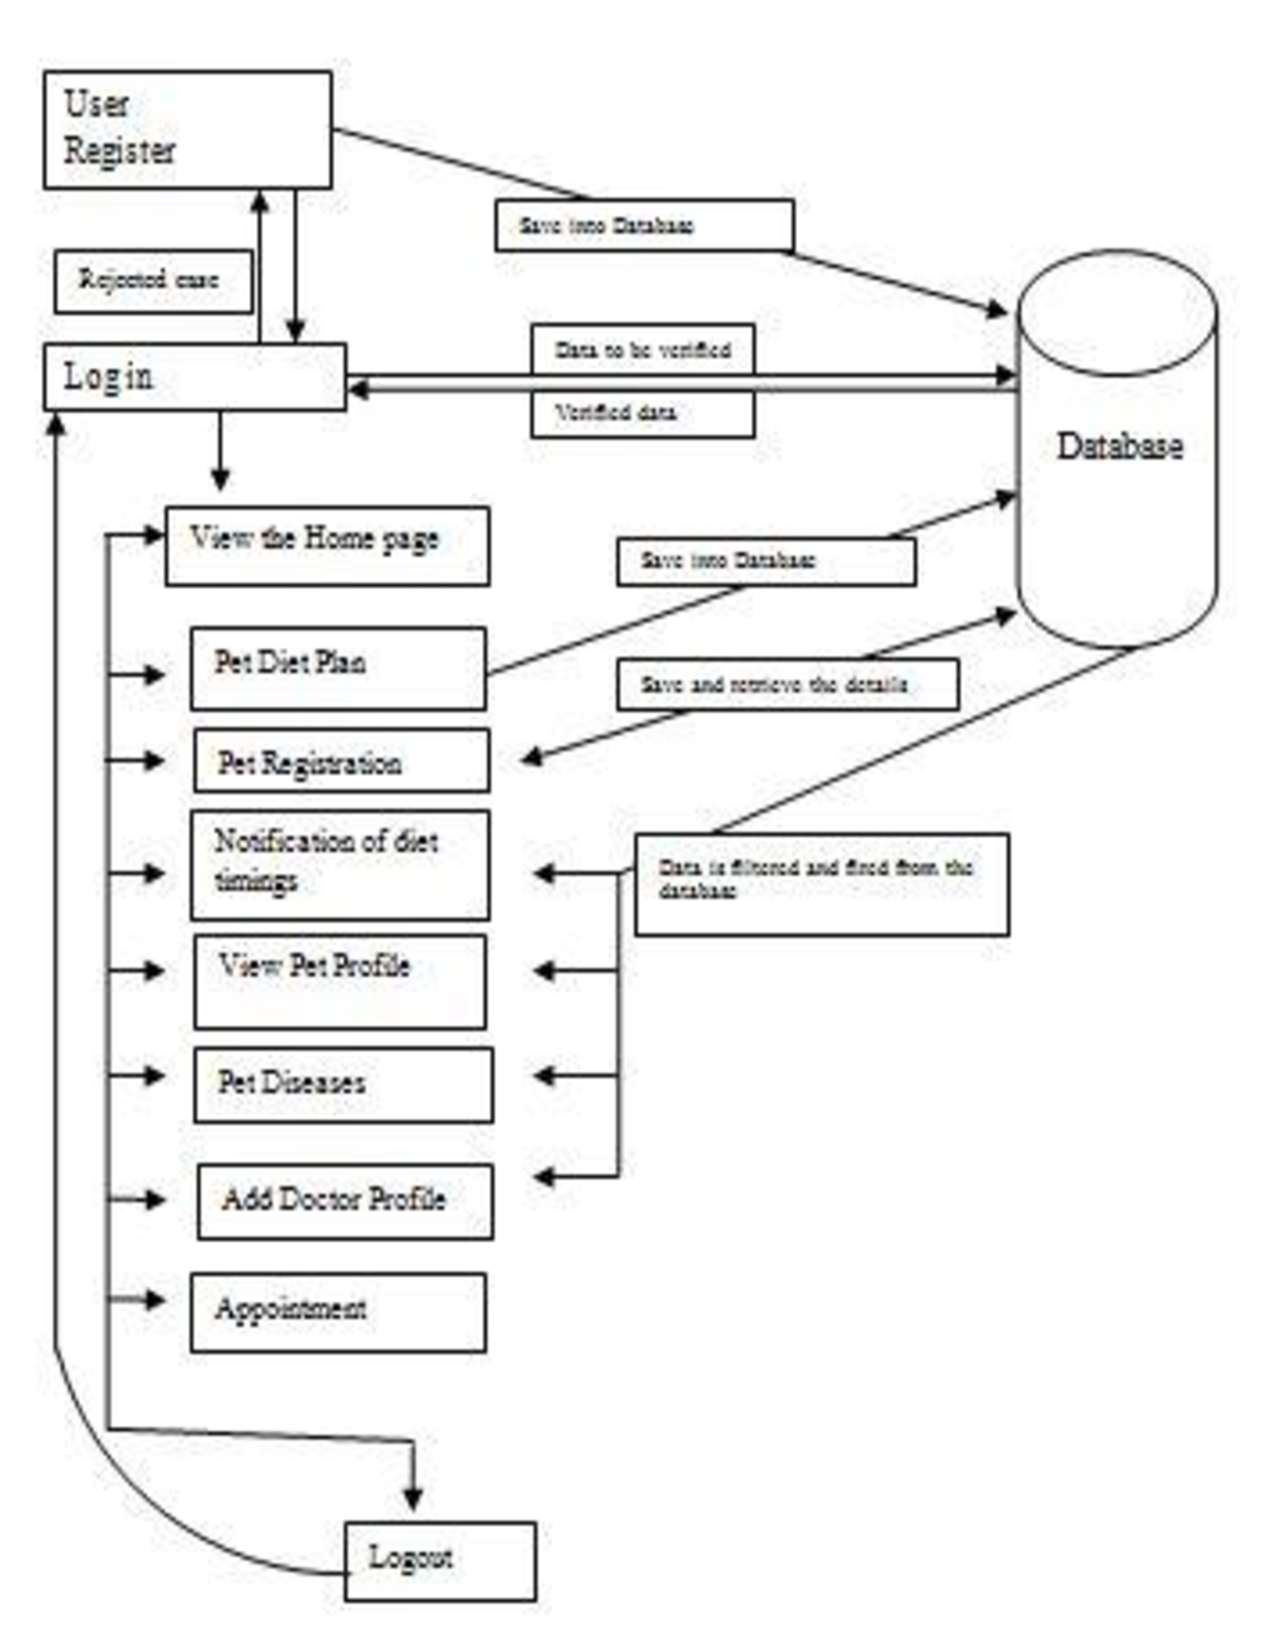
\includegraphics[scale=0.5]{fivethree}
  \caption{Activity Processing Logic}
\end{figure}
Website will only display the data which is provided by the Islamabad Pets & AVIAN Hospital G-10/4 sector. Website will handle and full fill the requirements of the hospital. Currently the website is displaying the Hospital information, services, doctors details and appointment facility.

\section{Application Access Security}
Cloud base database (firebase) which provides many services like secure authentication, push notification, cloud messaging, remote access, real time database etc. Security reasons, fast access and the reliable user authentication firebase database; used for this android project. Recently Gmail authentication is used for the user login in; later on other authentication methods might be used for the user access. 
\subsection{Database Security}
Firebase is a real time database which has separate security rules for user authentication, database and for the storage access. 

Database security rules are shown in below picture.

\begin{figure}[H]
 \centering
  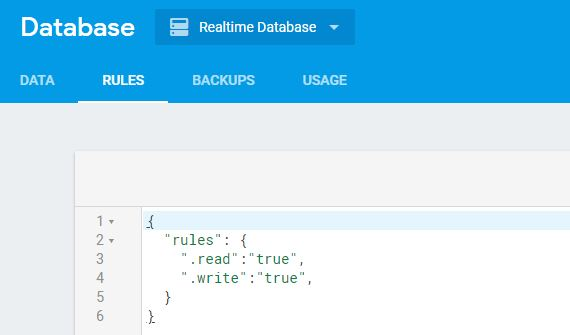
\includegraphics[scale=0.3]{asd}
  \caption{Firebase Database}
\end{figure}
	
Storage security rules are shown in below picture.
\begin{figure}[H]
\centering
 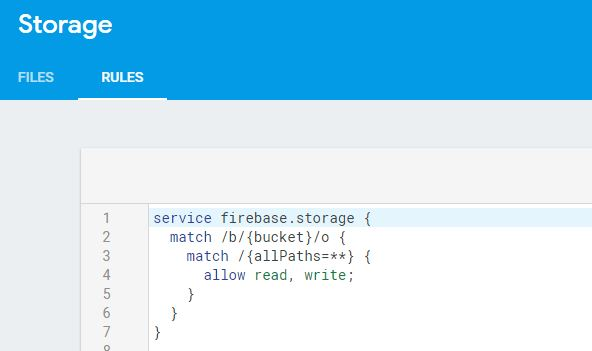
\includegraphics[scale=0.3]{dfg}
  \caption{Firebase Storage}
\end{figure}
Data is stored in the form of nodes into the JSON format. Unique keys or ids are created against each record. Security rules and creation of unique keys is a very handsome feature of firebase which make it different from other in aspect of authentication and database security.